\section{Theoretical aspects}

\emph{%
% 
This section treats the fundamentals of the theory of particle physics.
% 
Only topics that are deemed relevant for the rest of this thesis are treated, and as such this section is by no means comprehensive.
%
First the standard model and its particles are generally introduced, followed by \tk{todo}.
% 
For a more comprehensive, accessible overview of particle physics, the reader is referred to Ref.~\cite{griffiths}, and for mathematical formulations of underlying symmetries and the derivations of the Feynman rules to Ref.~\cite{peskin}.
}

% ____________________________________________________________________________
\subsection{The standard model}

The standard model (SM), widely recognized as one of the greatest successes of particle physics, is the physics model that summarizes, to the best of our knowledge, the particles that exist in nature, and how they interact with one another.
% 
Its predictions are consistent with many experiments performed in the second half of the 20${}^\text{th}$ century at scales extending over several orders of magnitude.
% 
The discovery~\cite{Aad:2012tfa,Chatrchyan:2012xdj,Chatrchyan:2013lba} of a particle compatible with the SM Higgs boson at the CERN LHC completed an important of the puzzle of the SM, the mechanism behind the masses of the intermediate vector bosons.
% 
Its conception is the result of decades of monumental effort from both the experimental and theoretical particle physics communities.


The SM is a quantum field theory (QFT); more specifically, it is a \textit{renormalizable} and \textit{locally invariant gauge theory}, meaning the fields $\psi$ are invariant under local gauge transformations.
% 
Its particles and interactions are encapsulated in the \textit{SM Lagrangian density} $\lagrangiansm$ (from here on referred to as simply the \textit{SM Lagrangian}), whose full, lengthy description can be found in Ref.~\cite{todo}.
% 
The SM Lagrangian fulfills the requirements of local gauge invariance and renormalizability, but it is by no means the only Lagrangian to do so.
% 
The form of the SM Lagrangian is `derived' (not in the mathmatical sense) from our knowledge of non-relativistic quantum mechanics, symmetry considerations, and from experiment.
% 
It is not a result of some underlying principles of QFT; it is instead postulated in such a way to fit experimental observations.


In principle, deriving the physics of electromagnetic, strong, and weak interactions is then as simple as solving the equation of motion, which much like in classical mechanics is derived from the least-action principle:
% 
\begin{linenomath*}
\begin{equation}
\label{eq:eom}
\partial_\mu \left(
    \frac{
        \partial \lagrangian
        }{
        \partial \left( \partial_\mu \psi \right)
        }
    \right)
    -
    \frac{\partial\lagrangian}{\partial\psi}
    = 0
\end{equation}
\end{linenomath*}
% 
where $\mu$ is in index to the four dimensions of spacetime, $\partial_\mu$ is shorthand for $\frac{\partial}{\partial x^\mu}$, i.e. the spacetime derivative with respect to the coordinate $x^\mu$, and $\psi$ (shorthand for $\psi(x^\mu)$) is a field.
% 
For a theory with multiple fields (as is the case for the SM), Equation~(\ref{eq:eom}) is supposed to hold for each field individually.
% 
Unfortunately, there is no easy solution to the equation of motion of the SM Lagrangian, and we need to resort to perturbative expansion to find approximate solutions, which is no trivial matter even for the simplest of particle physics processes.
% 
The full treatment of this perturbative expansion is beyond the scope of this text, and the reader is referred to the excellent treatment of this topic in Ref.~\cite{peskin}.
% 
In short, the perturbative expansion can be simplified to a sum of wonderfully descriptive \textit{Feynman diagrams}, which represent the terms of the perturbative expansion, and the \textit{Feynman rules}, which map the diagrams to an evaluable formulaic form.


Although undeniably a great success, the SM comes with a number of important `gaps'.
% 
For example, it lacks a description of gravity, highlighting the largest incompatibility of the SM with the theory of general relativity.
% 
Furthermore a description of dark matter and energy is lacking, and the observed matter-antimatter imbalance in the universe is also unexplained.
% 
These problems highlight some gaps in our description of naturally observed phenomena, but also on a more theoretical level there are aspects of the SM that are, for lack of a better word, uncomfortable.
% 
Overlooking for the moment the problem of massive neutrinos, the SM Lagrangian has 19 parameters that are, to the best of our knowledge, arbitrary.
% 
Although their experimentally determined values are used in SM predictions, there is no satisfying underlying theory explaining these parameters, which include for example the quark and lepton masses and the coupling constants of the electromagnetic, strong, and weak interactions.
% 
Given that the universe would look profoundly different under reasonably small variations of the values of these parameters~\cite{Cahn:1996ag}, it is a big open question how the parameters ended up having the values they do.
% 
% In fact, it is not even understood why there are 3 generations of leptons and quarks, rather than just 1, or any other number.


The particles encoded in SM Lagrangian can be categorized into quarks, leptons, gauge bosons, and the Higgs boson.
% 
The quarks come in 6 flavors, which are further categorized into 3 generations: the up and down quark (the first generation), the strange and the charm quark (the second generation), and the bottom and the top quark (the third generation).
% 
The up, charm, and top quarks carry an electric charge $q = 2/3e$ (where $e$ is the elementary electric charge), whereas the down, strange, and bottom quarks carry $q=-1/3$.
% 
Each quark comes in 3 `colors', typically denoted red, blue and green; the color of a quark is to be understood as yet another property of the quark, and has nothing to do with the notion of color in colloquial use.
% 
Every quark has a corresponding antiquark which comes in 3 anticolors and carries an opposite electric charge.
% 
The leptons come in 3 generations as well: the electron $\electron^-$, the muon $\muon^-$ and the tau $\taulepton^-$, and their associated neutrinos, $\neutrino_\electron$, $\neutrino_\muon$, and $\neutrino_\taulepton$ respectively.
% 
The corresponding antileptons carry opposite electric charge; the antiparticle of the electron is typically referred to as a \textit{positron}.
% 
The gauge bosons are the mediators of the three fundamental forces in the SM---the photon being the mediator of the electromagnetic interaction, the vector bosons $\wboson^+$, $\wboson^-$, and $\zboson$ the mediators of the weak interaction, and the gluon $\gluon$ (of which there are 8) the mediator of the strong interaction.
% 
The final particle is the Higgs boson, unlike the other bosons a spin-0 particle, which through the Higgs mechanism gives the vector bosons their mass.
% 
All the SM particles are summarized once more in Fig.~\ref{fig:particles}.

\begin{figure}[hbtp]
  \begin{center}
    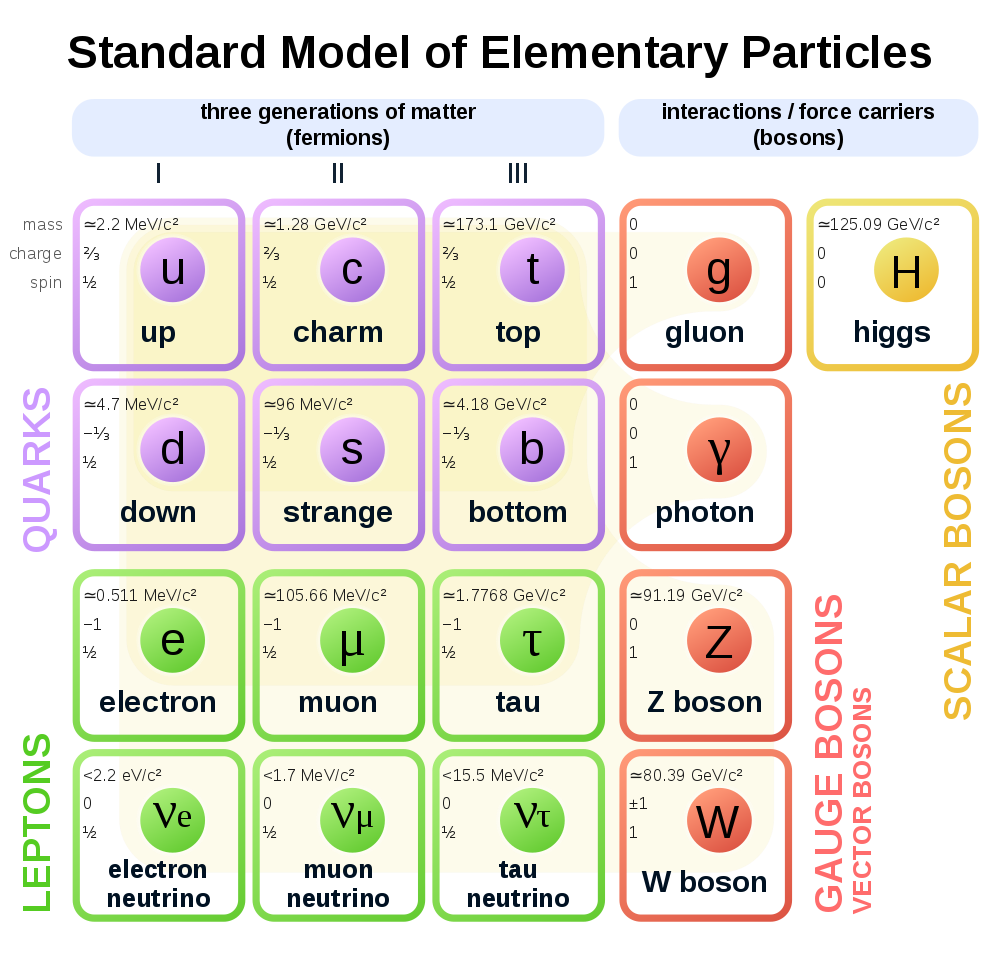
\includegraphics[width=0.7\linewidth]{img/theory/particles.png}
    \caption{
        Summary of the particles in the SM.
        % 
        THe quarks, leptons, gauge bosons and the Higgs boson are displayed in purple, green, red and yellow cells, respectively, sorted along generations for the fermions.
        % 
        Each cell contains three numbers in the top-left corner, corresponding to the mass, electric charge, and spin of the particle.
        % 
        Taken from Ref.~\cite{particles-wikicommons}.
        }
    \label{fig:particles}
  \end{center}
\end{figure}




% ____________________________________________________________________________
\subsection{Quantum chromodynamics}

The SM Lagrangian for QCD is~\cite{griffiths}
% 
\begin{linenomath*}
\begin{equation}
\lagrangian_\text{QCD} =
    i \overline{\psi_j} \gamma^\mu \partial_\mu \psi_j
    - m_j \overline{\psi_j} \psi_j
    - \frac{1}{4\pi} F^{\mu\nu} F_{\mu\nu} 
    - g_s (\overline{\psi_j} \gamma^\mu t \psi) A_\mu
\,,
\end{equation}
\end{linenomath*}
% 
where $\psi_j$ is a field whose excitation corresponds to a quark of flavor $j$, $\gamma$ are the gamma matrices, $m$ is the mass of the quark, $F^{\mu\nu}$ is the gluon field strength tensor, $g_s$ is the coupling constant for QCD, $t$ are the Gell-Mann matrices, and $A^\mu$ are the gauge fields.
% 
A sum over each of the quark flavors $j$ is implied, and the color indices have been omitted.
% 
Besides the quark masses, the only parameter is $g_s$.
% 
It is related to what is commonly referred to as the \textit{strong coupling constant of QCD}:
% 
\begin{linenomath*}
\begin{equation}
\as = \frac{g_s^2}{4\pi}
\,.
\end{equation}
\end{linenomath*}
% 
% HIER VERDER: confinement, etc.


% ____________________________________________________________________________
\subsection{The Higgs mechanism}

\tk{TODO}




% ____________________________________________________________________________
\subsection{The Higgs boson transverse momentum spectrum}

\tk{TODO}



